\documentclass[aspectratio=169,11pt]{beamer}

\usepackage{amsmath}
\usepackage{array}
\usepackage{booktabs}
\usepackage{graphicx}
\usepackage{siunitx}
\usepackage{xcolor}
\usepackage{xurl}

\usetheme{Madrid}
\usecolortheme{default}
\setbeamertemplate{navigation symbols}{}
\setbeamertemplate{footline}[frame number]
\graphicspath{{assets/}}
\urlstyle{same}

\newcommand{\good}[1]{\textcolor{green!45!black}{#1}}
\newcommand{\warn}[1]{\textcolor{red!65!black}{#1}}
\newcommand{\blue}[1]{\textcolor{blue!65!black}{#1}}
\newcommand{\pathtext}[1]{{\scriptsize\url{#1}}}
\newcommand{\src}[1]{\vfill{\tiny\textcolor{gray!75!black}{Source: \url{#1}}}}
\newcolumntype{L}[1]{>{\raggedright\arraybackslash}p{#1}}
\newcolumntype{R}[1]{>{\raggedleft\arraybackslash}p{#1}}

\title[NN Fitting Results]{Production MLP Fitting Results}
\subtitle{\(\Delta P^{0.5}\) Stage-3 anchor-off five seeds and seed42 trajectory diagnostics}
\author{Linan Jiang}
\institute{Aalto University}
\date{21 May 2026}

\begin{document}

\begin{frame}
  \titlepage
\end{frame}

\begin{frame}{Current Model}
\small
\begin{block}{Production model}
This deck now reports the true production MLP: Stage-3 \texttt{anchor\_off},
seeds 7/17/42/99/2024, warm-started from the Stage-2 winner and refined on raw
CDF supervision.
\end{block}

\begin{block}{Inputs and scaling}
\footnotesize
The current variant is \texttt{a\_dp050\_plus\_pressures}. Inputs include
normalized time, tilt, plume count, injection duration, control backpressure,
and log injection/chamber pressure. The target is still scaled with
\[
A=(\Delta P)^{0.5}\rho_a^{-0.25}d_n^{0.5}.
\]
\end{block}

\begin{block}{Reading boundary}
\footnotesize
The five-seed mean is the thesis result. Seed42 is the lowest-RMSE production
MLP seed and is used only for diagnostic plots.
\end{block}
\end{frame}

\begin{frame}{Full-Clean Result}
\small
\begin{tabular}{L{0.34\linewidth}R{0.14\linewidth}R{0.14\linewidth}R{0.14\linewidth}R{0.14\linewidth}}
\toprule
Model & RMSE & MAE & Bias & P95 \\
\midrule
Production MLP mean(5) & \good{4.735 \(\pm\) 0.037} & 3.293 \(\pm\) 0.039 & +0.626 & 9.167 \\
Production MLP seed42 & \good{4.689} & 3.251 & +0.486 & 9.092 \\
SVGP Stage-3 seed42 & \blue{4.628} & \blue{3.173} & -0.070 & 9.242 \\
\bottomrule
\end{tabular}

\vspace{0.7em}
\begin{tabular}{L{0.34\linewidth}R{0.16\linewidth}R{0.16\linewidth}R{0.18\linewidth}}
\toprule
Model & Cov1 & Cov2 & mean std \\
\midrule
Production MLP mean(5) & \good{0.867} & \good{0.985} & \SI{6.049}{mm} \\
Production MLP seed42 & 0.870 & 0.986 & \SI{6.032}{mm} \\
SVGP Stage-3 seed42 & 0.703 & 0.939 & \SI{4.000}{mm} \\
\bottomrule
\end{tabular}

\vspace{0.6em}
\footnotesize
The careful conclusion: MLP does not beat SVGP on RMSE/MAE, but its uncertainty
coverage is substantially more conservative.
\src{Thesis/generated/baseline_comparison_20260521/headline_full_clean.csv}
\end{frame}

\begin{frame}{Evaluation Size}
\small
\begin{columns}[T,onlytextwidth]
\begin{column}{0.48\linewidth}
\begin{tabular}{L{0.58\linewidth}R{0.30\linewidth}}
\toprule
Item & Value \\
\midrule
CSV files & 2,754 \\
Trajectories & \num{24316} \\
Prediction points & \num{692942} \\
Truth range & \SIrange{0.00}{95.88}{mm} \\
Time window & \SIrange{0}{5}{ms} \\
\bottomrule
\end{tabular}
\end{column}
\begin{column}{0.48\linewidth}
\begin{block}{Representative seed42}
\footnotesize
\begin{itemize}
  \item RMSE = \SI{4.689}{mm}
  \item MAE = \SI{3.251}{mm}
  \item Bias = +\SI{0.486}{mm}
  \item P95 absolute error = \SI{9.092}{mm}
  \item 1\(\sigma\)/2\(\sigma\) coverage = 0.870 / 0.986
\end{itemize}
\end{block}
\end{column}
\end{columns}
\src{MLP/eval/rmse_eval_clean_20260521_123603_distill_cdf_onset_v2_ablate_anchor_off_20260521_123126/metrics_summary.json}
\end{frame}

\begin{frame}{Predicted vs. Measured Penetration}
\centering
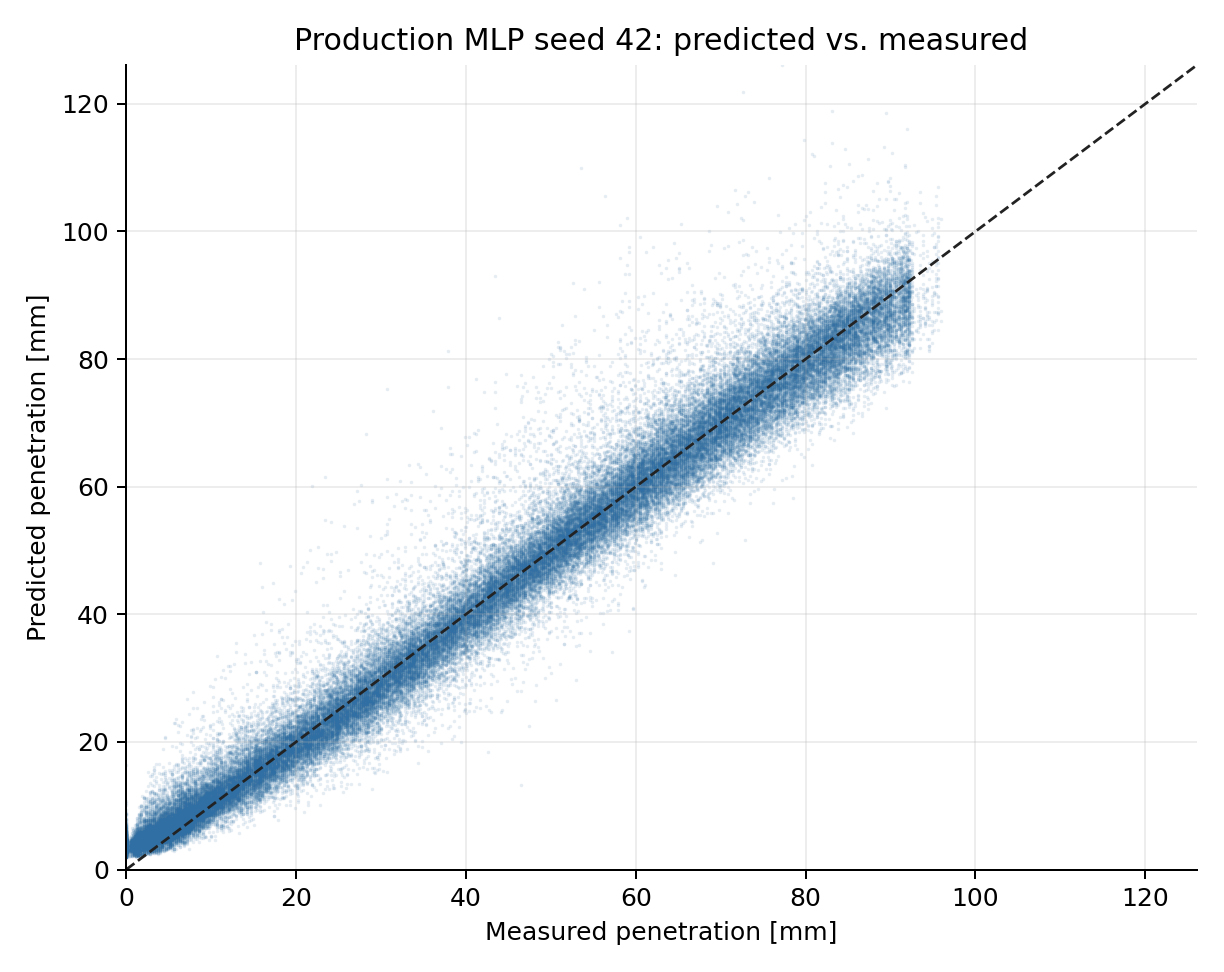
\includegraphics[width=0.78\linewidth,height=0.76\textheight,keepaspectratio]{pred_vs_actual_seed42.png}
\src{Thesis/images/neural_network_fit_results_20260521/pred_vs_actual_seed42.png}
\end{frame}

\begin{frame}{Residual Distribution}
\begin{columns}[T,onlytextwidth]
\begin{column}{0.58\linewidth}
\centering
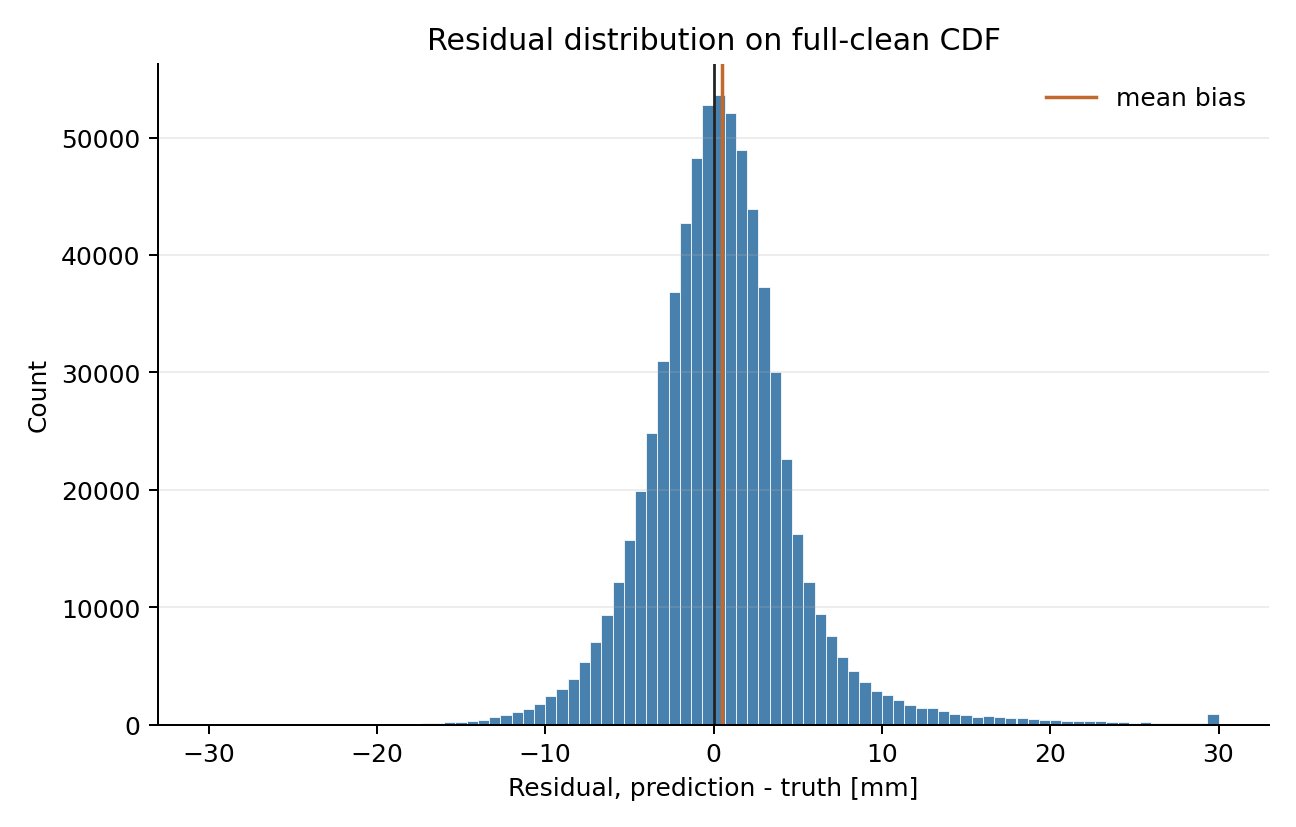
\includegraphics[width=\linewidth,height=0.72\textheight,keepaspectratio]{residual_histogram_seed42.png}
\end{column}
\begin{column}{0.38\linewidth}
\small
\begin{block}{Residual definition}
\[
e=\hat y_{\mathrm{pen}}-y_{\mathrm{pen}}.
\]
\end{block}
\begin{itemize}
  \item seed42 bias is +\SI{0.486}{mm}, small relative to RMSE.
  \item P95 absolute error is \SI{9.092}{mm}.
  \item 2\(\sigma\) coverage is 0.986, above the Gaussian nominal 0.954.
\end{itemize}
\end{column}
\end{columns}
\end{frame}

\begin{frame}{Five-Seed Repeatability}
\centering

\includegraphics[width=0.86\linewidth,height=0.72\textheight,keepaspectratio]{production_mlp_per_seed_rmse.png}
\src{Thesis/images/neural_network_fit_results_20260521/production_mlp_per_seed_rmse.png}
\end{frame}

\begin{frame}{Per-Folder RMSE}
\centering
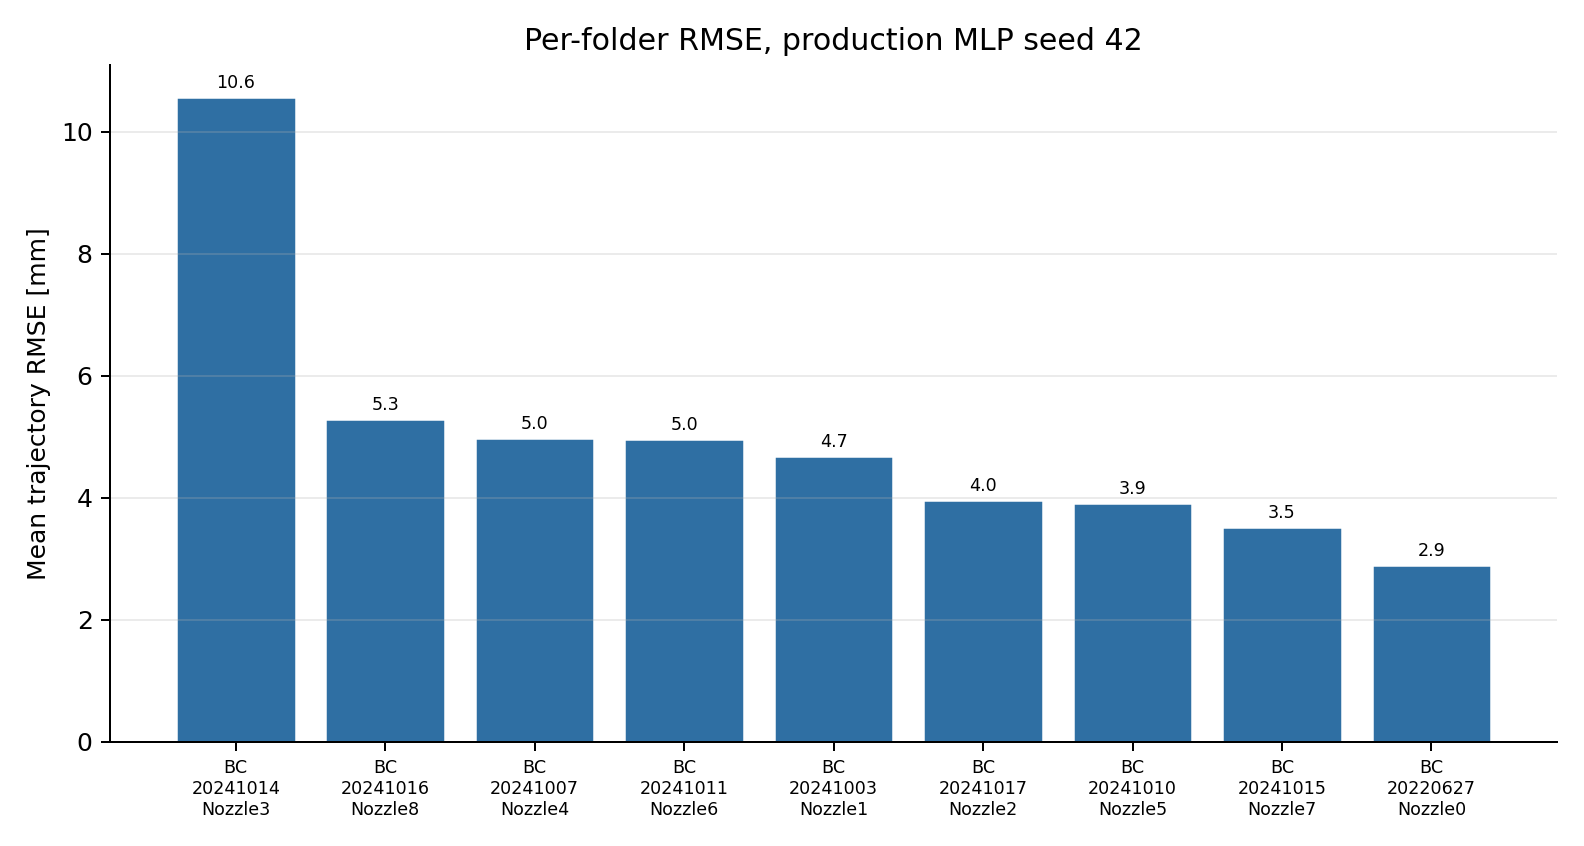
\includegraphics[width=0.92\linewidth,height=0.74\textheight,keepaspectratio]{per_folder_rmse_seed42.png}
\src{MLP/eval/rmse_eval_clean_20260521_123603_distill_cdf_onset_v2_ablate_anchor_off_20260521_123126/per_folder.csv}
\end{frame}

\begin{frame}{Per-Folder Coverage}
\centering

\includegraphics[width=0.92\linewidth,height=0.74\textheight,keepaspectratio]{per_folder_coverage_seed42.png}
\src{MLP/eval/rmse_eval_clean_20260521_123603_distill_cdf_onset_v2_ablate_anchor_off_20260521_123126/per_folder.csv}
\end{frame}

\begin{frame}{Representative Trajectories}
\begin{columns}[T,onlytextwidth]
\begin{column}{0.50\linewidth}
\centering

\includegraphics[width=\linewidth,height=0.66\textheight,keepaspectratio]{best_traj_seed42.png}

\footnotesize
Nozzle0 T4 plume 0: RMSE \SI{0.382}{mm}, coverage 1.00 / 1.00.
\end{column}
\begin{column}{0.50\linewidth}
\centering
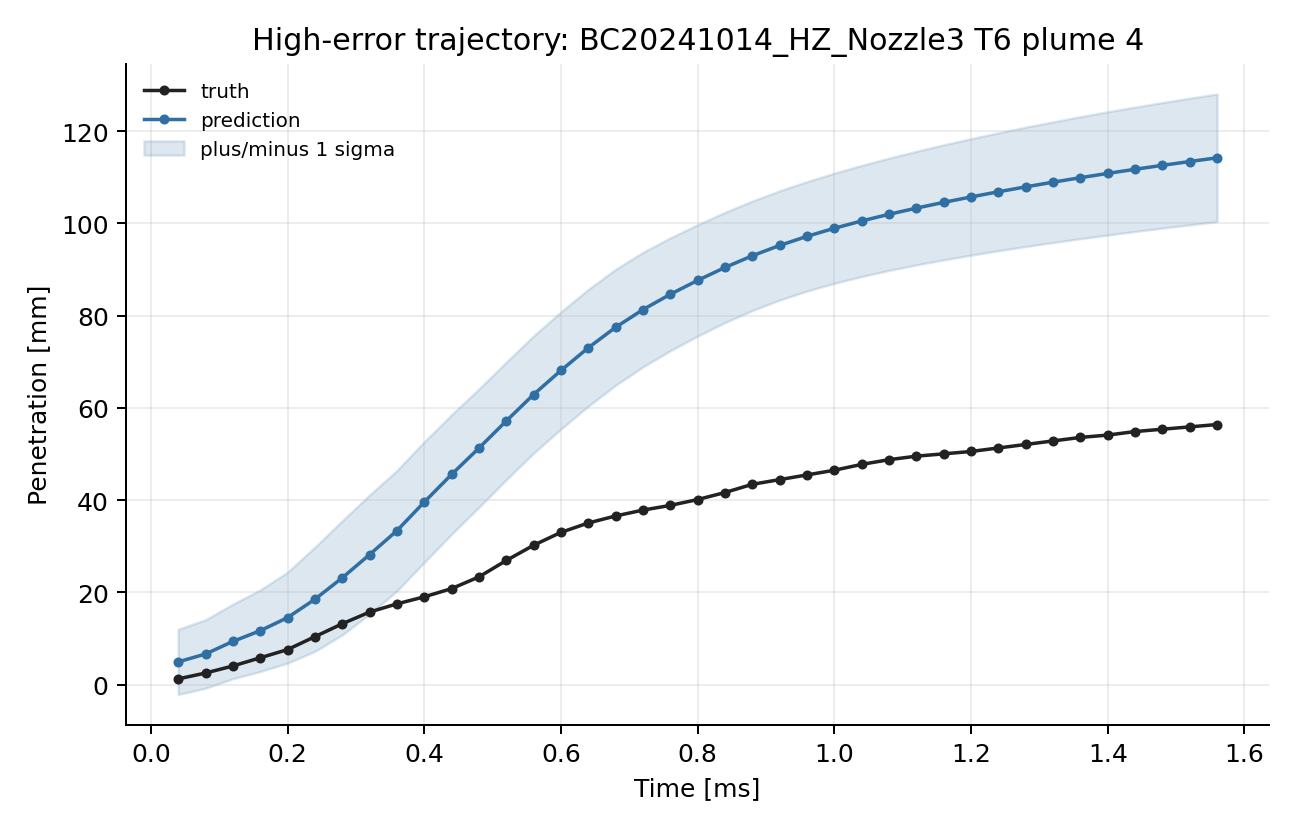
\includegraphics[width=\linewidth,height=0.66\textheight,keepaspectratio]{worst_traj_seed42.png}

\footnotesize
Nozzle3 T6 plume 4: RMSE \SI{42.763}{mm}, coverage 0.205 / 0.282.
\end{column}
\end{columns}
\src{Thesis/generated/neural_network_fit_results_20260521/summary.json}
\end{frame}

\begin{frame}{Residual Risk}
\small
\begin{enumerate}
  \item \good{Overall fitting is stable:} five-seed full-clean RMSE is \(4.735\pm0.037\) mm.
  \item \good{Uncertainty is conservative:} this is acceptable for a screening surrogate.
  \item \warn{Nozzle3 remains the main failure mode:} it has the highest per-folder RMSE and weak worst-trajectory coverage.
  \item \warn{Do not claim a full MLP win over SVGP:} SVGP still has slightly better full-clean RMSE/MAE.
\end{enumerate}

\begin{block}{Thesis phrasing}
\footnotesize
Production MLP closes the gap to SVGP while providing more conservative
uncertainty coverage, and it clearly outperforms HA/NS empirical curve baselines.
\end{block}
\end{frame}

\begin{frame}{File Index}
\small
\begin{tabular}{L{0.28\linewidth}L{0.62\linewidth}}
\toprule
Item & File \\
\midrule
Slides source & \pathtext{Thesis/slides/neural_network_fit_results_slides_en/neural_network_fit_results_slides_en.tex} \\
Figures & \pathtext{Thesis/images/neural_network_fit_results_20260521/} \\
Figure script & \pathtext{Thesis/generated/neural_network_fit_results_20260521/make_figures.py} \\
Representative seed eval & \pathtext{MLP/eval/rmse_eval_clean_20260521_123603_distill_cdf_onset_v2_ablate_anchor_off_20260521_123126/} \\
5-seed aggregate & \pathtext{Thesis/generated/baseline_comparison_20260521/production_mlp_full_clean_per_seed.csv} \\
\bottomrule
\end{tabular}
\end{frame}

\end{document}
